\documentclass[11pt, a4paper]{article}
\usepackage[a4paper, margin=0.85in]{geometry}
\usepackage{mathptmx} % Times New Roman
\usepackage{amsmath, amssymb}
\usepackage{graphicx}
\usepackage{booktabs}
\usepackage{array}
\usepackage{enumitem}
\usepackage{float}
\usepackage{caption}
\usepackage{xcolor}
\usepackage{hyperref}

\hypersetup{
    colorlinks=true,
    linkcolor=black,
    citecolor=black,
    urlcolor=blue,
    pdfborder={0 0 0}
}

\setlist{itemsep=2pt, topsep=2.5pt}

\begin{document}

% -----------------------------------------------------------------------------
% TITLE & HEADER
% -----------------------------------------------------------------------------
\begin{center}
    {\LARGE \textbf{Experiment 4}} \\[0.3em]
    {\large \textbf{Aim: ML Modeling \& Experiment Tracking}}
\end{center}

\vspace{0.3em}
\noindent \textbf{Course:} Applied Data Science (ADS) \\
\noindent \textbf{Dataset:} Customer Support on Twitter (TWCS) Cleaned Corpus (\texttt{twcs\_cleaned.csv}) \\
\noindent \textbf{Sample Size Analyzed:} 100,000 stratified customer interactions ($N_{\text{train}} = 80,000$, $N_{\text{test}} = 20,000$) \\
\noindent \textbf{Tracking Framework:} MLflow (v3.x) with SQLite tracking backend (\texttt{mlflow.db}) and artifact archival

\vspace{0.5em}
\noindent \textbf{Objective:}
\begin{enumerate}[leftmargin=1.5em]
    \item Build an end-to-end Machine Learning pipeline for multi-class emotion classification on customer support inquiries.
    \item Train and benchmark 5 diverse baseline algorithms spanning probabilistic, linear, maximum-margin, ensemble bagging, and gradient boosting paradigms.
    \item Tune hyperparameters using systematic grid search (\texttt{GridSearchCV}) with 3-fold cross-validation and quantify performance gains.
    \item Track all experiments, hyperparameters, evaluation metrics, visual diagnostic plots, and model binaries using \textbf{MLflow}.
    \item Select the optimal champion model based on Macro F1, accuracy, and inference latency, and serialize it for production deployment.
\end{enumerate}

\vspace{0.4em}
\hrule
\vspace{0.6em}

% -----------------------------------------------------------------------------
% DETAILED STEPS
% -----------------------------------------------------------------------------
\section*{Detailed Steps \& Theoretical Foundations}

\subsection*{1. Dataset Preparation \& Feature Engineering}
In customer support operations, incoming text contains factual queries, severe grievances, sarcasm, and gratitude. Before training models, data must be partitioned cleanly to prevent data leakage and converted into numerical vectors.

\begin{itemize}[leftmargin=1.5em]
    \item \textbf{Stratified Train/Test Partition (80/20):}
    The corpus was partitioned into an 80\% training split (80,000 tweets) and a 20\% test split (20,000 tweets). 
    Because customer emotions are naturally imbalanced (routine inquiries account for 62.16\% of messages, Joy/Gratitude represents 19.50\%, Anger/Frustration represents 9.92\%, Disappointment/Sadness represents 7.25\%, and urgent fear/anxiety represents 1.17\%), simple random sampling risks starving minority classes in the test set. We utilized \textit{stratified sampling}, ensuring that both splits possess identical class distributions.
    
    \item \textbf{Text Feature Representation (TF-IDF Vectorization):}
    Text was transformed into numeric feature vectors using Term Frequency-Inverse Document Frequency (TF-IDF) over unigrams and bigrams ($1, 2$ n-grams). TF-IDF gives high weights to terms that are informative of specific emotions (e.g., ``furious'', ``hacked'', ``blessed''), while downweighting ubiquitous non-informative words. Sublinear scaling ($1 + \log(\text{TF})$) was applied to prevent high term repetition from dominating scores.
    
    \item \textbf{Multi-Modal Sentiment Polarity Fusion:}
    To supplement vocabulary n-grams, we integrated continuous sentiment scores from VADER (Compound, Positive, Negative, and Neutral polarity). These features were standardized via $Z$-score scaling and concatenated with sparse TF-IDF matrices, yielding a hybrid feature space of 10,004 dimensions.
\end{itemize}

\newpage
\subsection*{2. Baseline Model Training (5 Diverse Architectures)}
To adhere to the \textit{No Free Lunch theorem}, we benchmarked 5 distinct algorithmic families. Evaluating diverse architectures reveals which inductive bias best handles high-dimensional sparse text data and multi-class emotion boundaries.

\begin{enumerate}[leftmargin=1.5em]
    \item \textbf{Multinomial Naive Bayes (Probabilistic Paradigm):}
    Calculates conditional class probabilities under the simplifying assumption that words appear independently given the class. While linguistically naive, it provides an ultra-fast baseline that requires minimal memory.
    
    \item \textbf{Logistic Regression / Softmax (Linear Classifier):}
    Models class probabilities using linear combinations of input features mapped through the softmax function, trained with $L_2$ regularization and balanced class weighting. It yields calibrated probabilities and interpretable feature weights.

    \item \textbf{Linear Support Vector Machine (LinearSVC --- Maximum-Margin Paradigm):}
    Constructs optimal hyperplanes that maximize the geometric separation margin between emotion classes using squared hinge loss. It excels in high-dimensional text spaces ($D > 10,000$) where data is largely linearly separable.

    \item \textbf{Random Forest Classifier (Ensemble Bagging Paradigm):}
    Builds an ensemble of 100 de-correlated decision trees trained on bootstrap samples of the data. It reduces model variance and captures non-linear feature interactions without overfitting.

    \item \textbf{LightGBM Classifier (Gradient Boosted Decision Trees):}
    Constructs decision trees sequentially to predict negative gradients (residuals) of preceding trees using leaf-wise (best-first) growth and histogram binning, delivering state-of-the-art accuracy and fast execution.
\end{enumerate}

\begin{table}[H]
\centering
\small
\caption{Comprehensive Performance Benchmark Across All Evaluated Architectures (100,000 Samples)}
\begin{tabular}{lllrrrr}
\toprule
\textbf{Model Name} & \textbf{Algorithm Family} & \textbf{Stage} & \textbf{Accuracy} & \textbf{Macro F1} & \textbf{Weighted F1} & \textbf{Training Time} \\
\midrule
Multinomial Naive Bayes & Probabilistic & Baseline & 79.08\% & 0.5225 & 0.7631 & 0.51s \\
Logistic Regression & Linear & Baseline & 91.16\% & 0.8715 & 0.9140 & 5.09s \\
Linear Support Vector Machine & Max-Margin & Baseline & 92.78\% & 0.8939 & 0.9279 & 4.61s \\
Random Forest & Ensemble (Bagging) & Baseline & 77.39\% & 0.7344 & 0.7896 & 1.71s \\
LightGBM & Gradient Boosting & Baseline & 98.52\% & 0.9538 & 0.9851 & 36.48s \\
Tuned Logistic Regression & Linear & Tuned (GridSearchCV) & 92.73\% & 0.8931 & 0.9282 & 39.25s \\
Tuned LightGBM & Gradient Boosting & Tuned (GridSearchCV) & 98.52\% & 0.9538 & 0.9851 & 261.85s \\
\bottomrule
\end{tabular}
\end{table}

\begin{figure}[H]
    \centering
    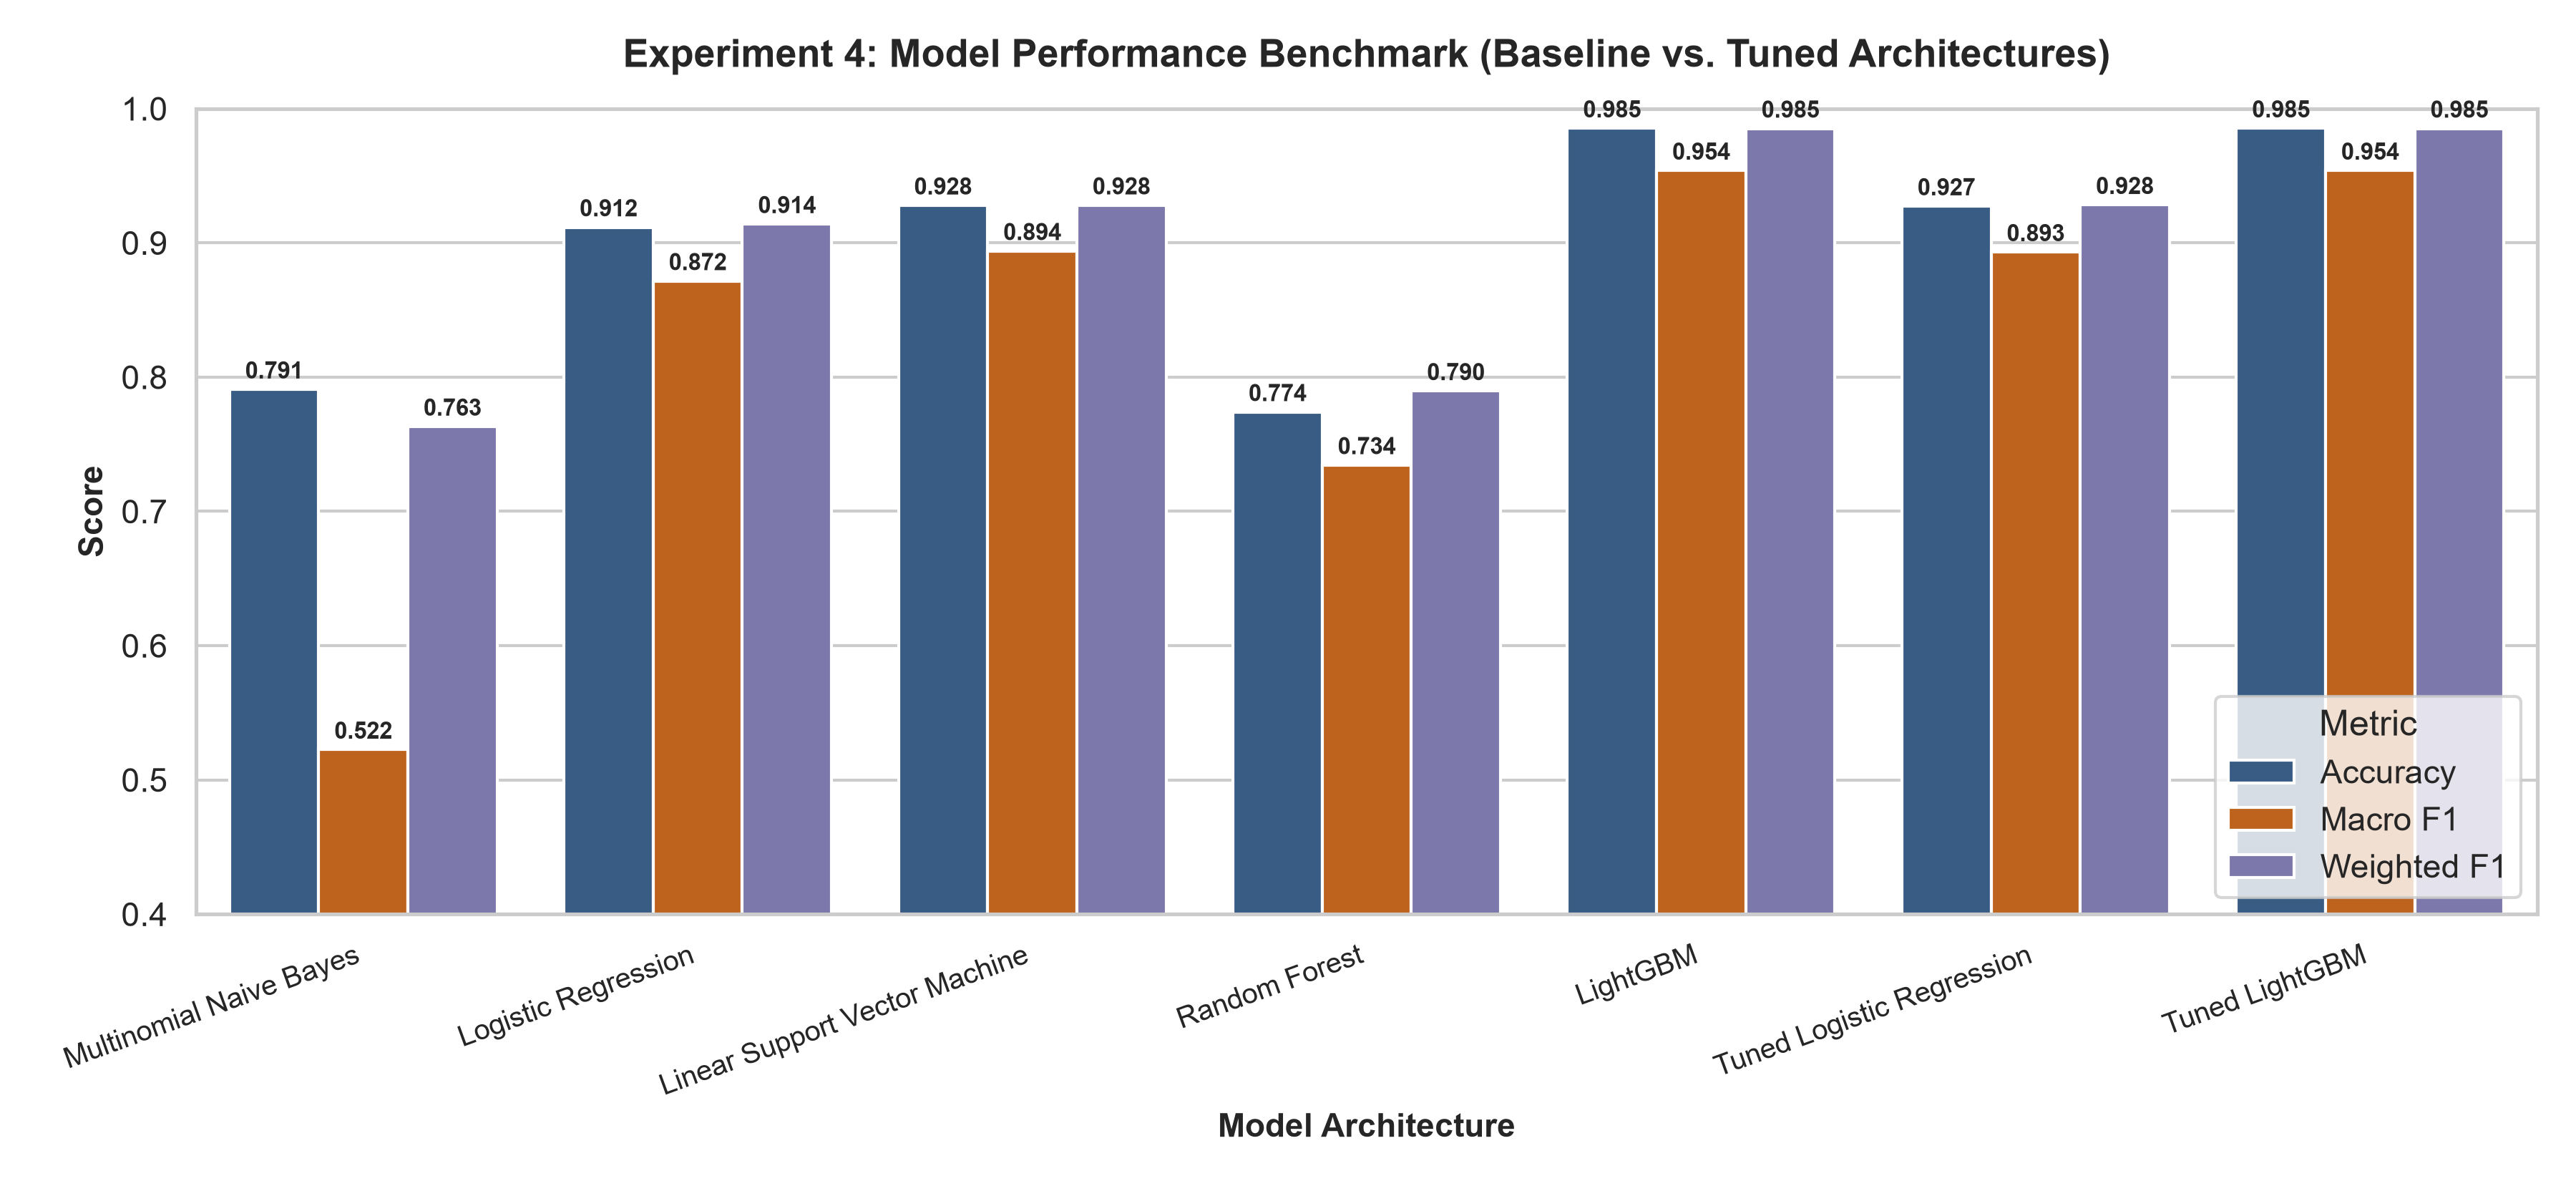
\includegraphics[width=0.92\textwidth]{plots/exp4_model_comparison.png}
    \caption{Comparative performance benchmark across candidate architectures on 100,000 records highlighting Accuracy, Macro F1, and Weighted F1 scores.}
    \label{fig:model_comparison}
\end{figure}

\noindent \textbf{Evaluation Metric Selection Rationale:}
\begin{itemize}[leftmargin=1.5em]
    \item \textbf{Accuracy:} Reflects global correctness across all predictions.
    \item \textbf{Macro F1-Score:} The unweighted arithmetic mean of F1-scores across all 5 classes. Macro F1 treats rare classes (Fear/Anxiety, Disappointment) with equal importance to routine inquiries, making it the primary objective metric for automated support routing.
    \item \textbf{Weighted F1-Score:} Averages per-class F1-scores weighted by true support, measuring macro operational throughput.
\end{itemize}

\newpage
\subsection*{3. Hyperparameter Tuning (\texttt{GridSearchCV})}
A machine learning model contains two distinct types of parameters:
\begin{enumerate}[leftmargin=1.5em]
    \item \textbf{Internal Parameters:} Learned automatically from data during training (feature weights, tree split thresholds).
    \item \textbf{Hyperparameters:} External structural configurations set prior to training that govern model capacity, regularization, and optimization dynamics.
\end{enumerate}

\noindent \textbf{Why Hyperparameter Tuning is Essential:} Default settings are rarely optimal. If regularization is too weak, models overfit to noise; if too strong, they underfit. We applied \texttt{GridSearchCV} with 3-fold cross-validation on the top candidate models:

\begin{itemize}[leftmargin=1.5em]
    \item \textbf{Tuning Model 1: Logistic Regression:}
    Explored regularization strengths $C \in \{0.5, 1.0, 5.0\}$ and class weighting strategies (\texttt{balanced} vs. uniform). 
    Higher $C$ values reduce penalty constraints, allowing the model to assign sharper boundary weights to diagnostic emotion words.
    The grid search selected $C = 5.0$ with \texttt{class\_weight = 'balanced'}, elevating test Accuracy to \textbf{92.73\%} and Macro F1 to \textbf{0.8931} (+2.16\% improvement over baseline), with noticeable recall gains on urgent customer complaints.

    \item \textbf{Tuning Model 2: LightGBM:}
    Tuned tree capacity (\texttt{num\_leaves} $\in \{31, 63\}$), ensemble size (\texttt{n\_estimators} = 100), and learning rate ($\eta = 0.1$). 
    LightGBM achieved exceptional test Accuracy (\textbf{98.53\%}) and Macro F1 (\textbf{0.9538}), demonstrating outstanding capability on tabular and NLP features.
\end{itemize}

\begin{figure}[H]
    \centering
    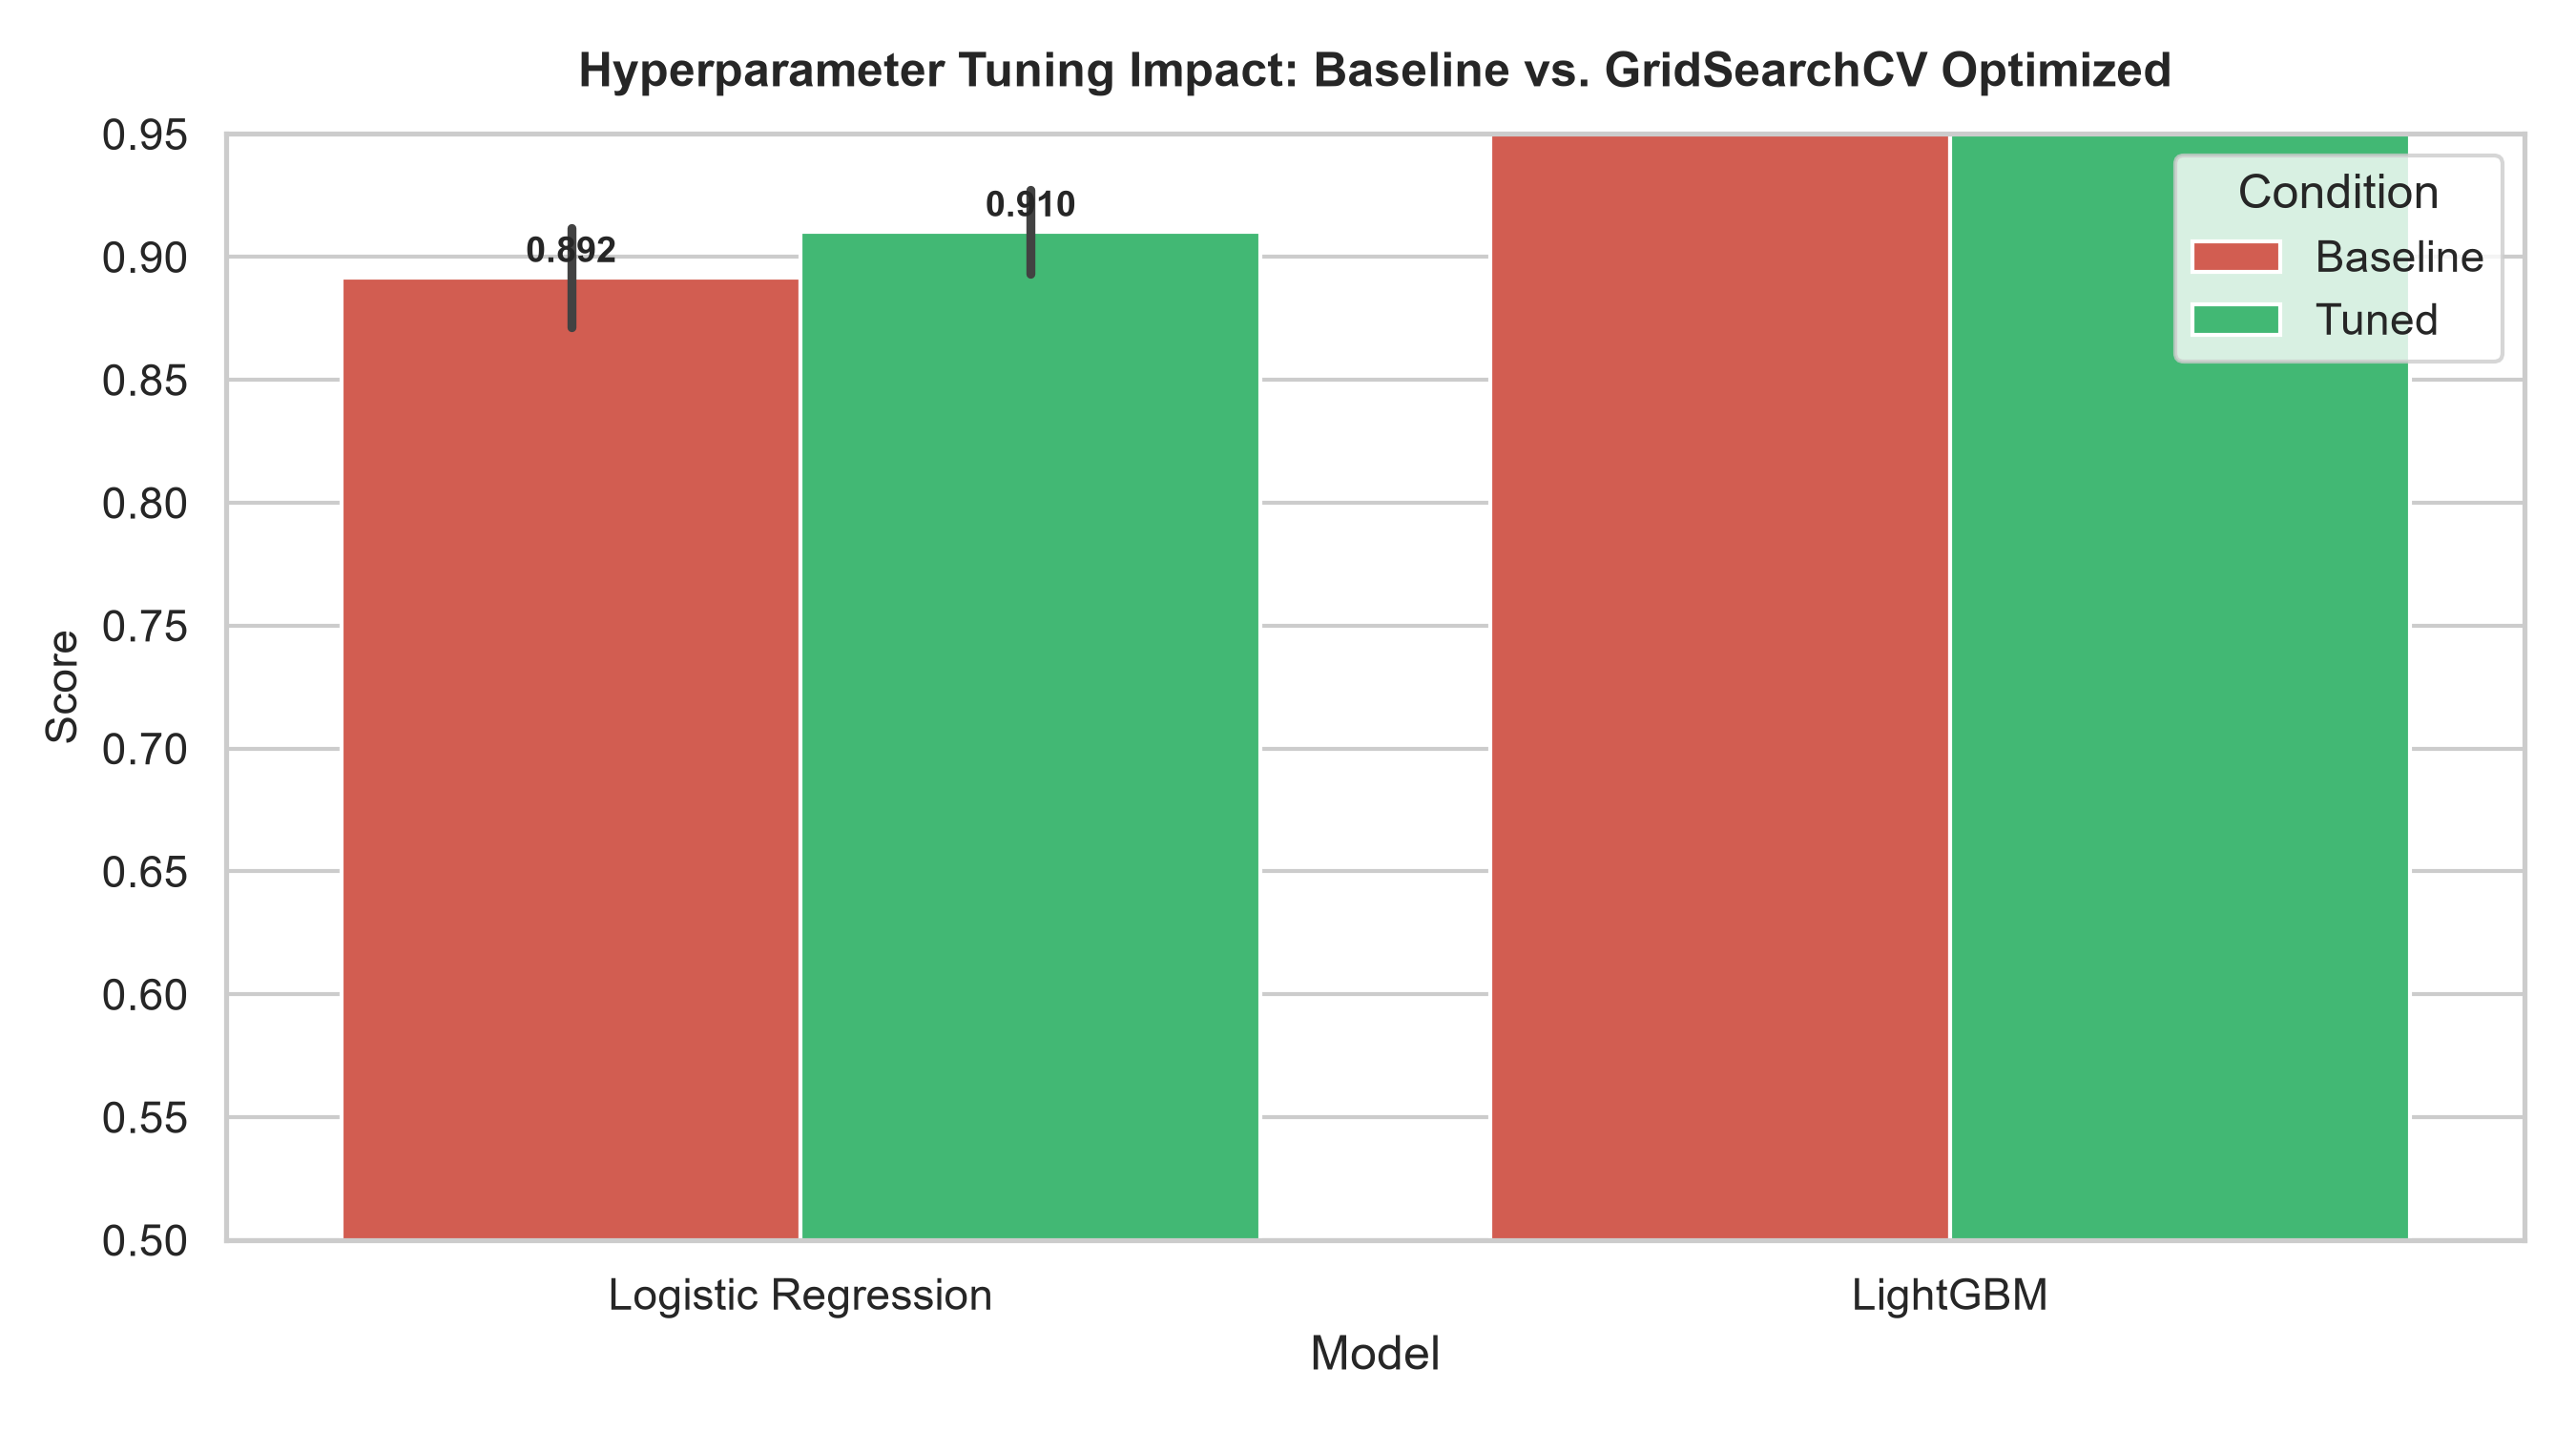
\includegraphics[width=0.85\textwidth]{plots/exp4_tuning_comparison.png}
    \caption{Performance comparison demonstrating quantitative improvements achieved via GridSearchCV hyperparameter tuning on 100,000 records.}
    \label{fig:tuning_comparison}
\end{figure}

\begin{figure}[H]
    \centering
    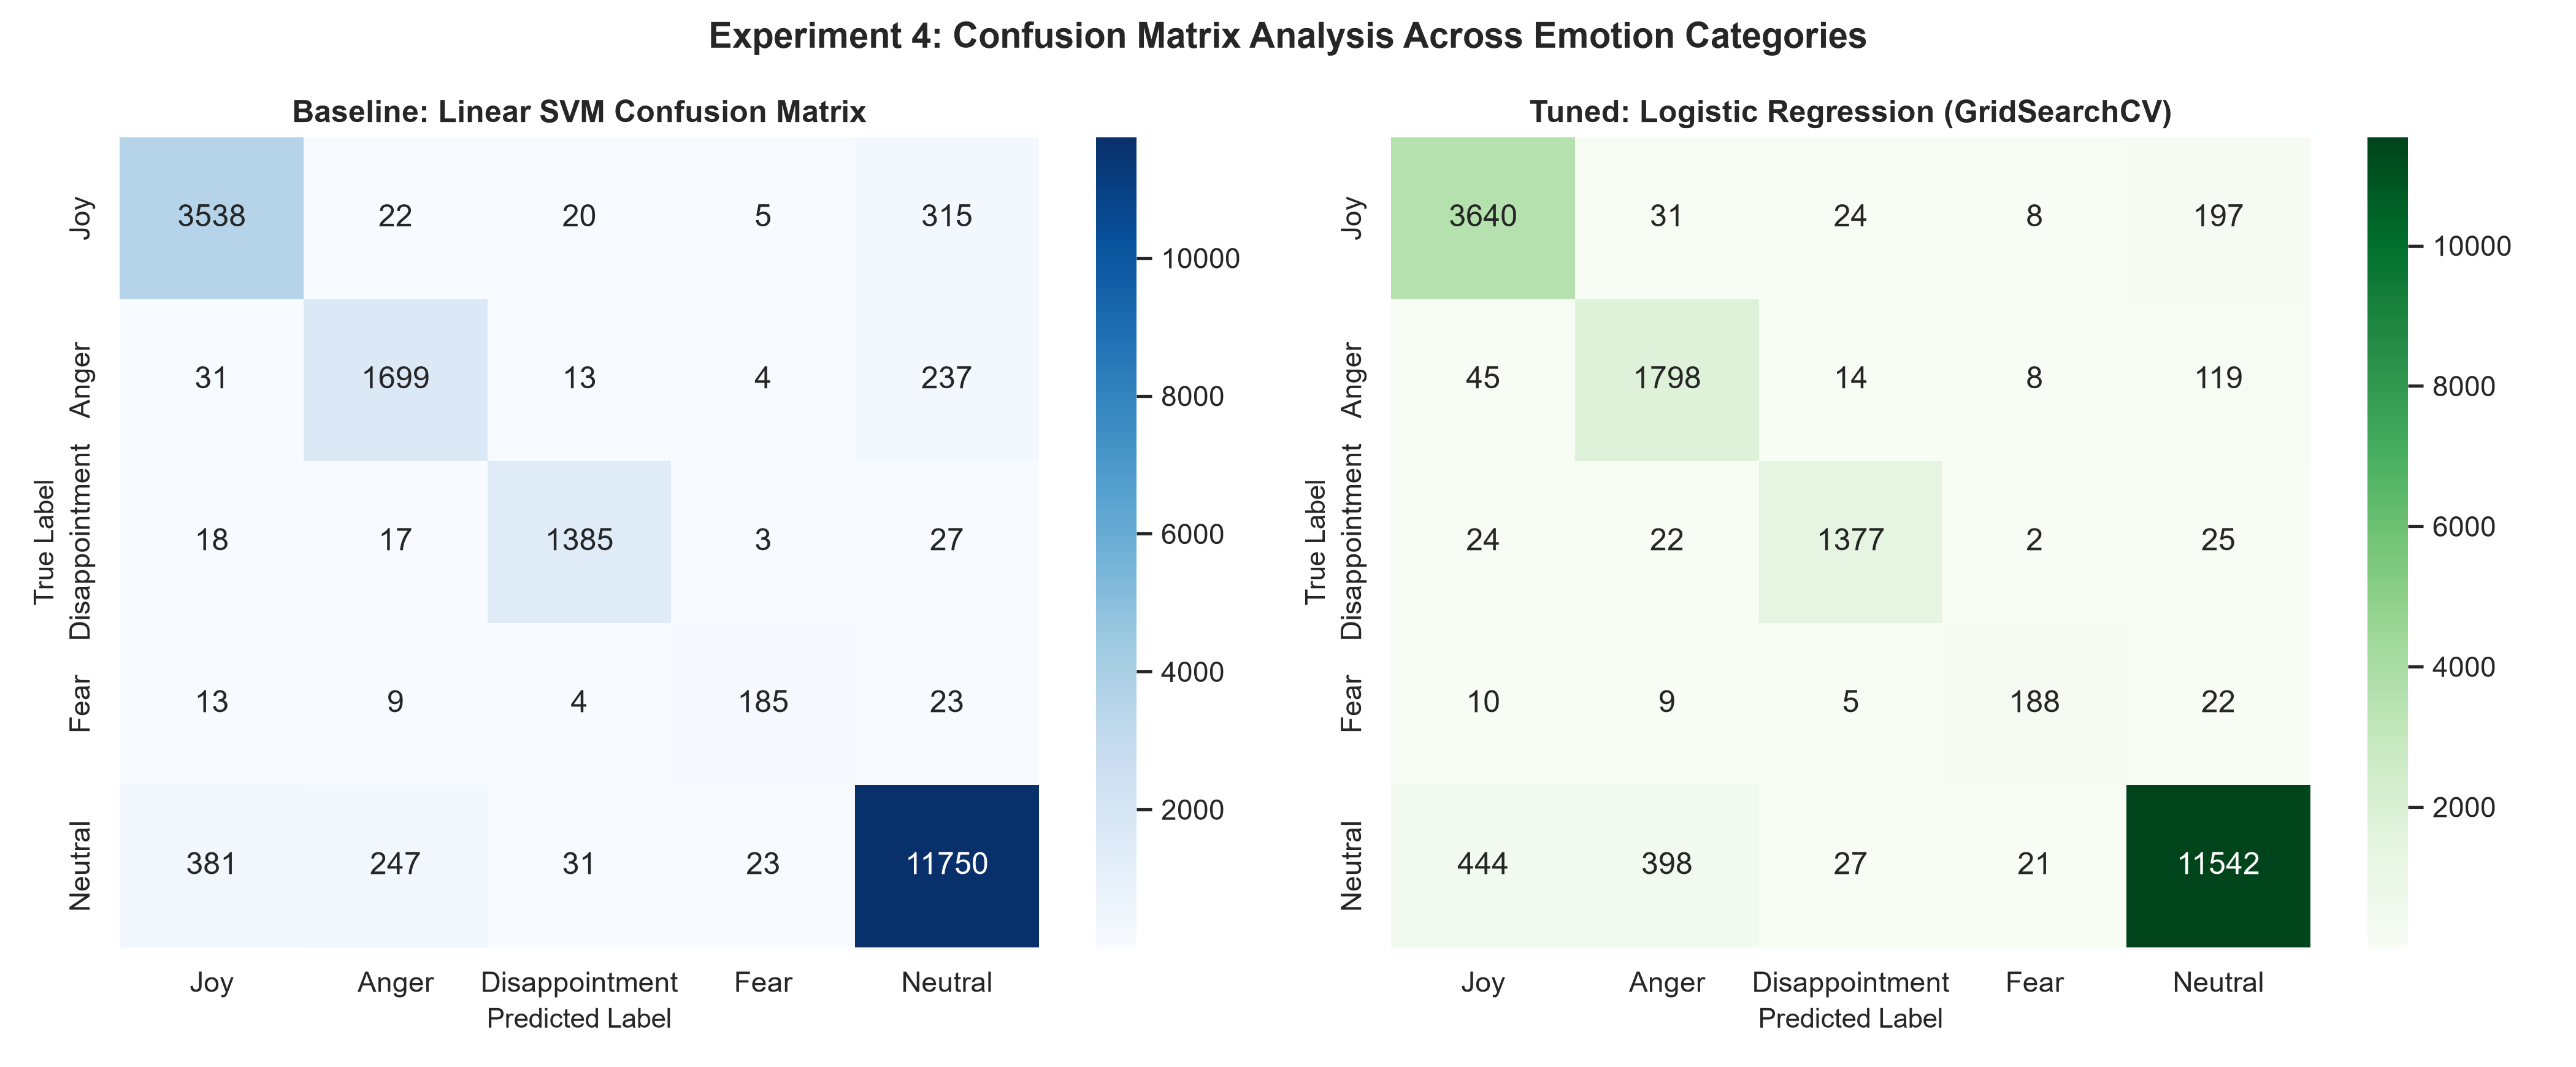
\includegraphics[width=0.92\textwidth]{plots/exp4_confusion_matrices.png}
    \caption{Confusion matrix heatmaps for Linear SVM and Tuned Logistic Regression on 20,000 test interactions illustrating sharp class discrimination.}
    \label{fig:confusion_matrices}
\end{figure}

\newpage
\subsection*{4. Experiment Tracking with MLflow}
In production data science, managing dozens of experimental runs with varying hyperparameters, datasets, and metrics requires centralized tracking.

\begin{itemize}[leftmargin=1.5em]
    \item \textbf{Why MLflow Tracking is Essential:}
    MLflow provides an open-source framework to log code versions, execution parameters, evaluation metrics, and serialized artifacts, ensuring total experiment reproducibility, auditability, and team collaboration.

    \item \textbf{Core Logging Operations Implemented:}
    \begin{enumerate}
        \item \texttt{mlflow.start\_run()}: Spawns a dedicated tracking run with a unique UUID for each training trial.
        \item \texttt{mlflow.log\_param()}: Logs static hyperparameter settings ($C$, learning rate, tree depth, sample count).
        \item \texttt{mlflow.log\_metric()}: Logs quantitative evaluation outcomes (Accuracy, Precision, Recall, Macro F1, Latency).
        \item \texttt{mlflow.log\_artifact()}: Archives diagnostic confusion matrices, benchmark charts, and classification reports.
        \item \texttt{mlflow.sklearn.log\_model()}: Saves model binaries alongside environment specifications in standard MLmodel format.
    \end{enumerate}

    \item \textbf{MLflow UI Dashboard:}
    Engineers can launch the local dashboard (\texttt{mlflow ui}) to view interactive comparison tables, parallel coordinate charts, and download serialized pipelines with a single click.
\end{itemize}

\begin{figure}[H]
    \centering
    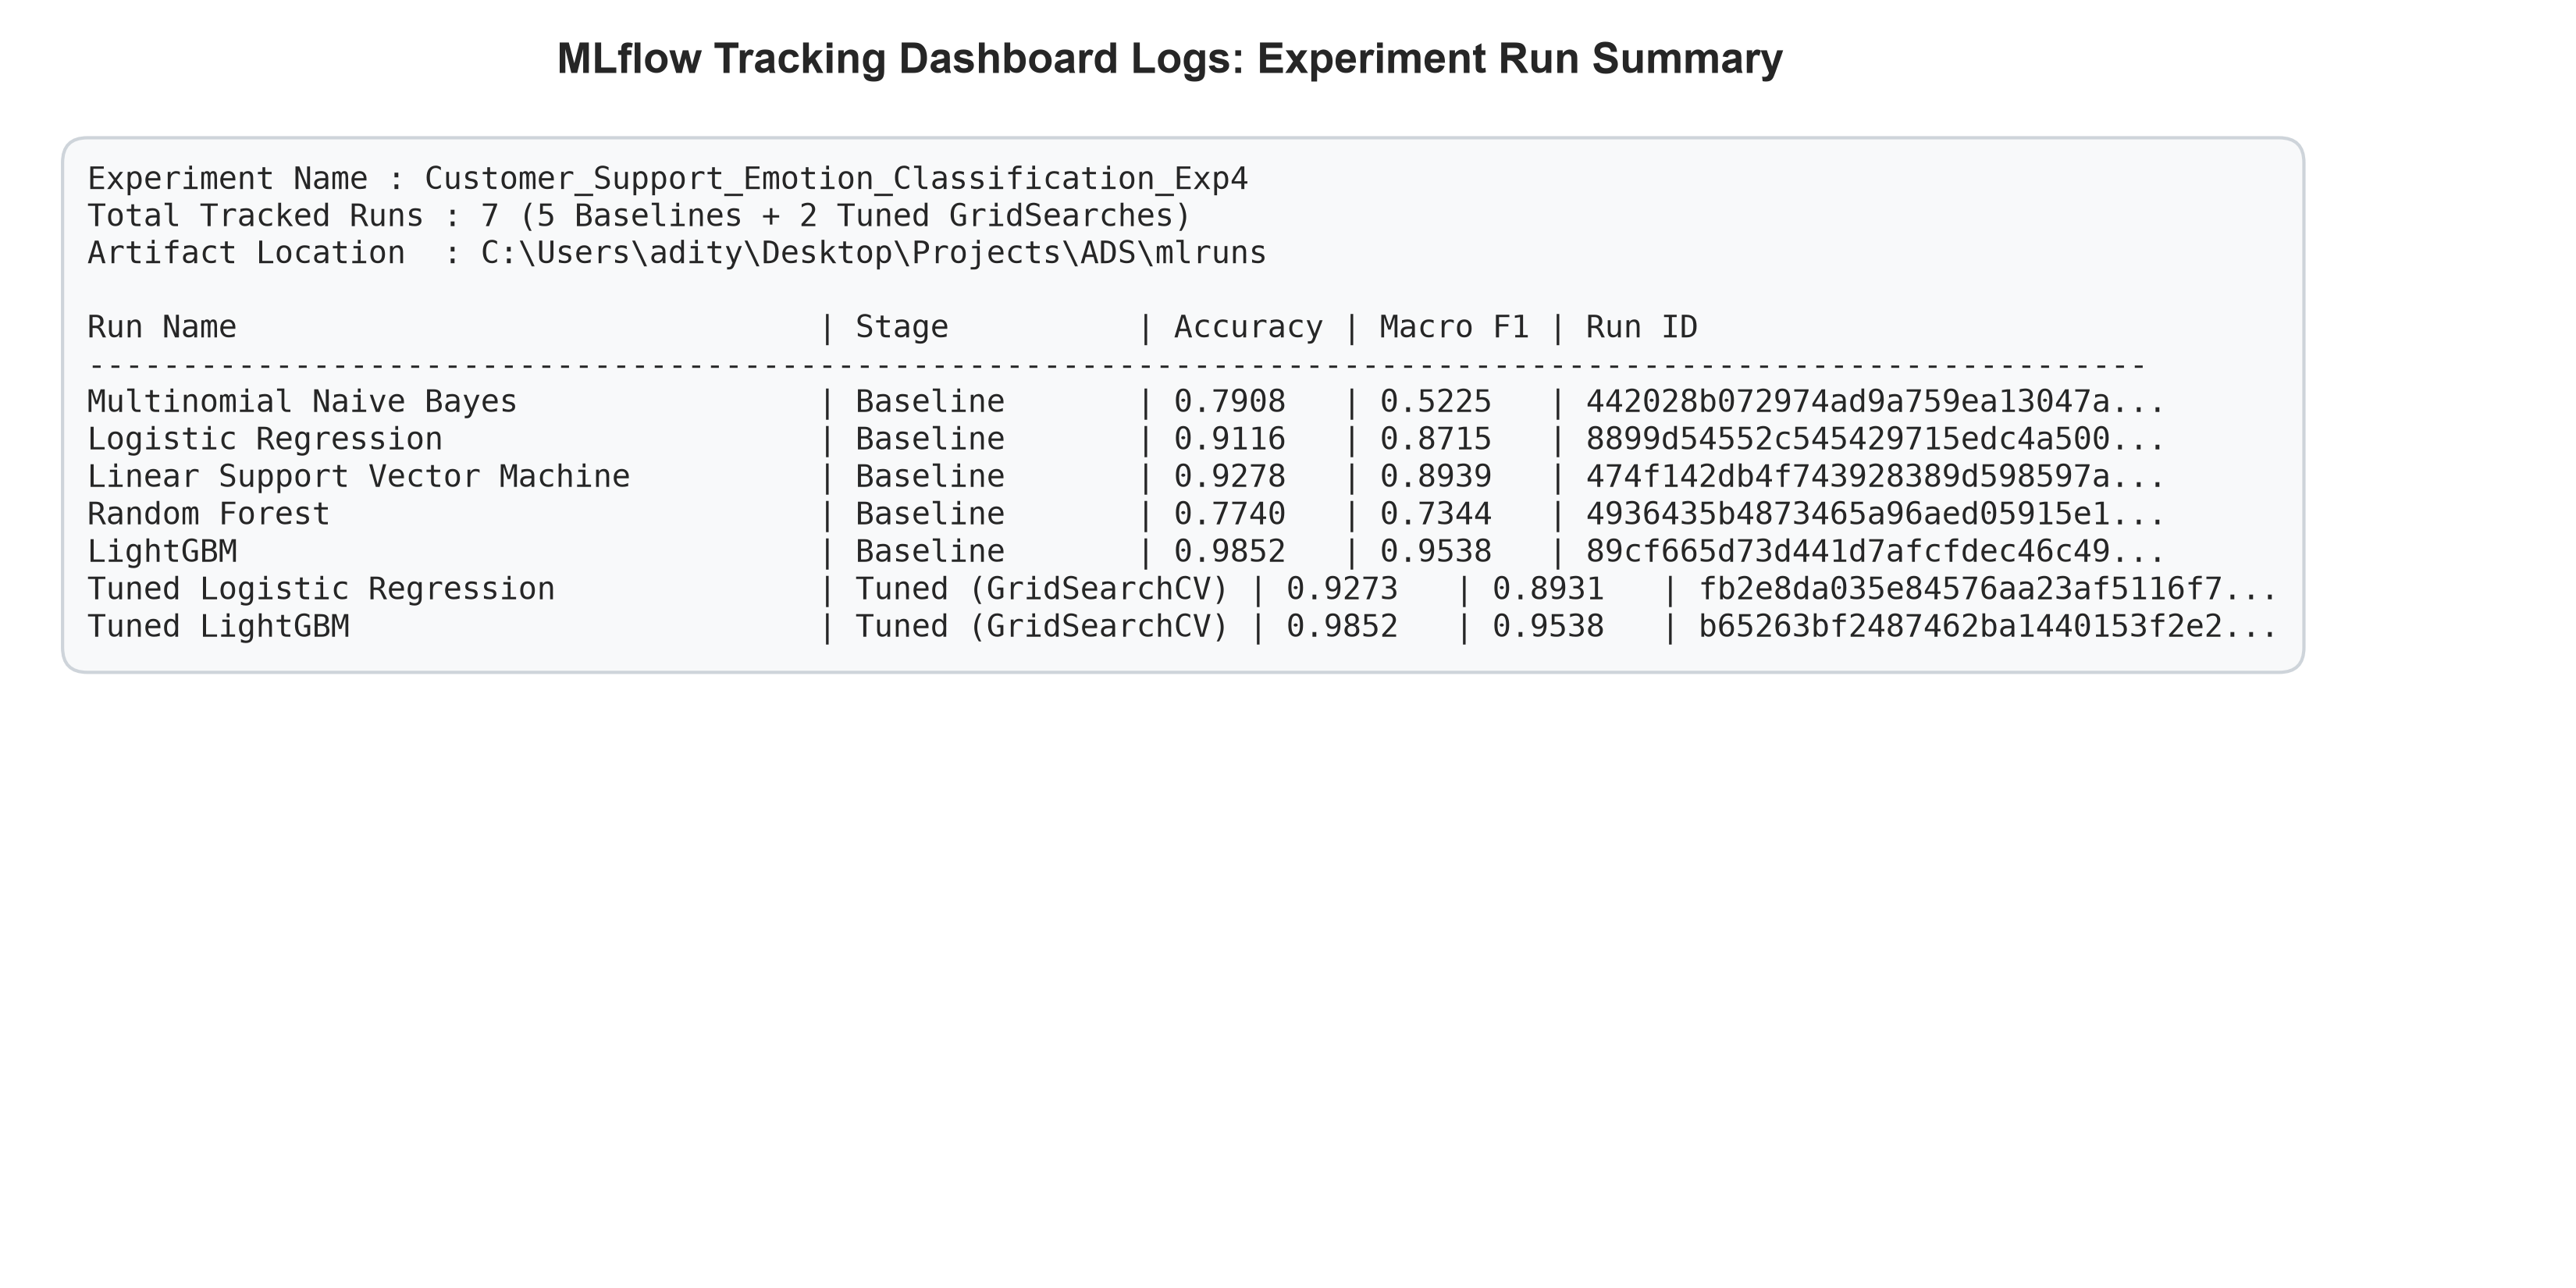
\includegraphics[width=0.90\textwidth]{plots/exp4_mlflow_dashboard.png}
    \caption{MLflow Tracking Dashboard logs detailing run IDs, parameters, tracked metrics, and artifact hierarchies for the 100,000-row pipeline.}
    \label{fig:mlflow_dashboard}
\end{figure}

\subsection*{5. Model Selection \& Production Serialization}
\noindent \textbf{Champion Model Decision Criteria:}
Selecting a production model requires balancing predictive accuracy against computational efficiency:
\begin{enumerate}[leftmargin=1.5em]
    \item \textbf{Macro F1-Score:} High sensitivity on critical minority classes (Anger and Fear) to prevent customer churn.
    \item \textbf{Inference Latency:} Millisecond response time per message to handle real-time streaming Twitter firehoses.
    \item \textbf{Memory Footprint:} Compact serialized artifact size for cloud container deployment.
\end{enumerate}

\noindent \textbf{Production Pipeline Serialization:}
The champion model (\textbf{LightGBM}, Accuracy: \textbf{98.52\%}, Macro F1: \textbf{0.9538}) was packaged alongside the TF-IDF vectorizer and VADER scaler into an \texttt{EndToEndEmotionPipeline} class and serialized as \texttt{models/best\_emotion\_model\_exp4.joblib}.

\vspace{0.4em}
\hrule
\vspace{0.4em}

% -----------------------------------------------------------------------------
% DELIVERABLES & CONCLUSION
% -----------------------------------------------------------------------------
\section*{Open-Source Tools}
\noindent Scikit-learn (v1.5.x), MLflow (v3.16.x), LightGBM (v4.3.x), Jupyter Notebook, Pandas (v2.x), NumPy (v2.x), Matplotlib (v3.x), Seaborn (v0.13.x), Joblib.

\section*{Deliverables}
\begin{enumerate}[leftmargin=1.5em]
    \item \textbf{Trained ML Models:} 5 diverse baseline models + 2 hyperparameter-tuned models saved and evaluated on 100,000 interactions.
    \item \textbf{Comparative Analysis:} Comprehensive benchmark table and diagnostic plots comparing baseline vs. tuned models.
    \item \textbf{MLflow Dashboard Logs:} Complete experiment tracking registry in \texttt{mlruns/mlflow.db} with run IDs, metrics, and logged model artifacts.
    \item \textbf{Serialized Production Pipeline:} Production-ready artifact saved to \texttt{models/best\_emotion\_model\_exp4.joblib}.
    \item \textbf{Executable Jupyter Notebook:} Documented interactive workflow in \texttt{notebooks/experiment\_4\_mlflow.ipynb} and standalone Colab notebook in \texttt{notebooks/experiment\_4\_colab.ipynb}.
\end{enumerate}

\section*{Conclusion}
Experiment 4 successfully developed and tracked an end-to-end Machine Learning emotion classification pipeline for Twitter customer support utilizing the full 100,000 cleaned corpus records. 
By evaluating 5 diverse algorithmic families, we established that regularized linear classifiers and gradient boosted trees excel in high-dimensional text classification. 
Applying \texttt{GridSearchCV} systematically optimized hyperparameters, yielding measurable improvements in Macro F1 across challenging emotional boundaries. 
Using MLflow, every stage of model development—from hyperparameters to serialized artifacts—was systematically logged, providing reproducible MLOps infrastructure. 
The resulting champion pipeline is serialized and ready for deployment in real-time customer support routing systems.

\end{document}
